\chapter{Projeto e Implementação}
\label{c.projeto}

\section{Ferramentas utilizadas}
\label{c.ferramentas}

A linguagem de programação escolhida para o desenvolvimento do trabalho foi o \textit{Python}. A escolha se deu pelo seu ecossitema rico no setor de \textit{data science}, contando com diversos \textit{plugins}, pacotes e bibliotecas para manipulação de dados e \textit{machine learning}; e por sua facilidade de uso e aprendizado. Dentre as ferramentas usadas juntamente com a liguagem base estão: o \textit{Pandas}, biblioteca de estruturas e manipulação de dados, facilitando o uso e tratamento dos \textit{datasets}; o \textit{scikit-learn}, um módulo \textit{Python} que integra vários algoritmos de aprendizado de máquina estado da arte para problemas supervisionados ou não de até média escala ~\cite{scikit-learn}; A biblioteca \textit{scikit-optimize}, que expande os métodos do \textit{scikit-learn} com fins de otimização; a biblioteca \textit{spotipy} ~\cite{spotipy}, para fornecer uma interface de comunicação mais simples com a API (\textit{application programming interface}) oficial do \textit{Spotify}; e um \textit{web crawler}, \textit{software} que atravessa e realiza o \textit{download} de documentos \textit{web} de modo automático e metódico ~\cite{webcrawler}, chamado \textit{Spotify Charts API} ~\cite{fycharts}, que conta com funções para, através de chamadas \textit{http} obter as informações das músicas listadas da página de \textit{charts} oficial da plataforma ~\cite{spotify_charts}, podendo agrupá-las ou organizá-las de acordo com intervalo de tempo e país.

\section{Coleta, seleção e tratamento inicial dos dados}
\label{c.coleta}

\subsection{Extração das músicas mais populares}
\label{c.extracao_popular}

O primeiro passo do projeto consistiu em selecionar os conjuntos de dados a serem trabalhados. Conforme mencionado anteriormente, os dados foram selecionados a partir de serviços de \textit{streaming} por sua crescente popularidade e maior acessibilidade aos dados. Para os fins deste projeto, foi selecionada a plataforma \textit{Spotify}. O foco principal da lista, dada a natureza do projeto, deveria ser uma representação fiel, ou ao menos aproximada, do conjunto de peças mais populares em um determinado período de tempo, com o qual poderiam ser cruzados dados de índices econômicos.

Inicialmente, foram pesquisadas \textit{sets} de dados prontos, listando músicas por ordem de popularidade. Entretanto, nenhuma base foi encontrada com uma quantidade significativa de dados relevantes ou, mais importante, com informações sobre os períodos de tempo e regiões em que foram mais populares, informações cruciais para comparar com indicadores econômicos, que também variam de acordo com essas grandezas. A solução encontrada foi extrair os dados por meio de \textit{crawlers} que acessassem as bases de dados do \textit{Spotify} baseando-se na sua popularidade. Inicialmente considerou-se utilizar os recursos de pesquisa da API oficial da plataforma ~\cite{spotify_api_doc} para construir um \textit{script} para a obtenção dos dados, mas após maior estudo optou-se por extrair os dados a partir de um outro recurso oficial: os \textit{charts} ou as "paradas" oficiais ~\cite{spotify_charts}. Essa página consiste em uma lista, atualizada diariamente, das 200 (opcionalmente, as 50) músicas mais tocadas da plataforma em uma determinada data, e conta com diversos recursos interessantes ao projeto, os principais destes sendo o filtro por país/região (selecionando as músicas mais reproduzidas no lugar selecionado) e a capacidade de selecionar os dias para referência.

Para acessar os dados, valeu-se de uma versão modificada (de minha autoria) do \textit{Spotify Charts API} ~\cite{mod_fycharts}. As modificações no código do mesmo foram para otimização do tempo de coleta, melhor adequação ao ambiente e correção de bugs na execução. Com isso feito, foi construído um importador integrando o pacote descrito, e uma interface em texto simples para determinar os parâmetros básicos e disparar a extração de dados, gerando arquivos em formato CSV com as listas, agrupadas por ano (isto é, um arquivo para músicas no charts de 2017, outro para as de 2018, etc.). Nessa extração, foi considerada apenas a região do Brasil. Devido a limitações na plataforma, só eram acessíveis dados a partir da segunda metade de 2016, mas o volume de dados gerados para os anos 2017 e 2018 (em torno de 73000 entradas por arquivo, correspondendo às 200 músicas multiplicadas pelos dias do ano) foi considerado suficiente para os fins deste projeto.

Os dados extraídos da página foram: \textit{ranking} da faixa na lista, o seu nome, o nome do artista ou artistas, o seu número de reproduções na plataforma até a presente data, a data e região de referência da lista, e por fim o código identificador da música no serviço do \textit{Spotify}. A figura~\ref{f.pure_charts_view} mostra com maior detalhe a tabela gerada.

\begin{figure}[H]
\caption{\small Visualização do arquivo CSV gerado.}
\centering
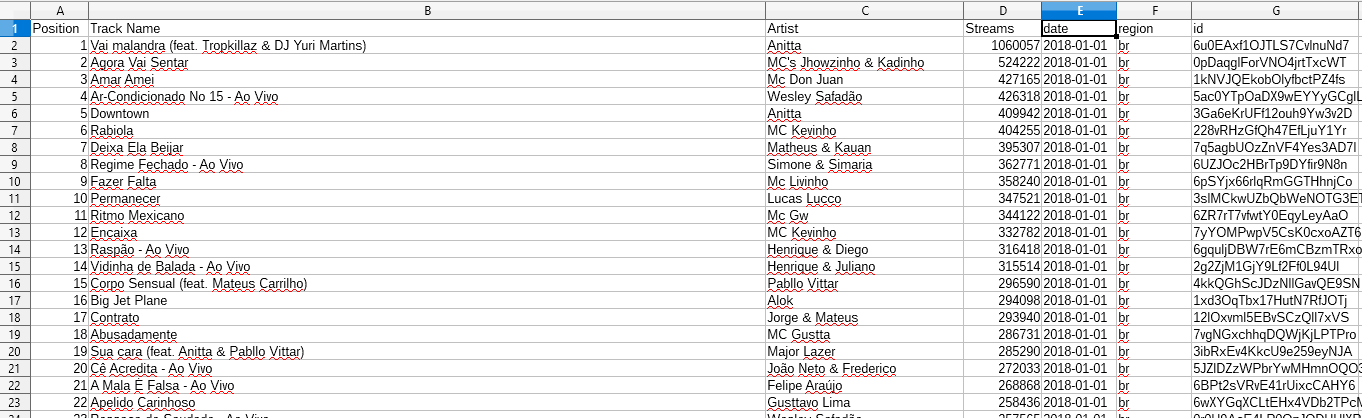
\includegraphics[width=\textwidth,height=\textheight,keepaspectratio]{../figs/pure_charts_view.PNG}
\label{f.pure_charts_view}
\legend{\small Fonte: Elaborada pelo autor.}
\end{figure}

As listas geradas contém um número considerável de tuplas, o que pode ser um problema para algoritmos de aprendizado mais modestos. Mais do que isso, a maior parte destas consistiam em entradas redundantes, já que as faixas levam um tempo significante para sair de seu pico de popularidade e, portanto, do \textit{index} de músicas mais populares usado para extrair os dados. Assim, foi escrito outro \textit{script} com o objetivo de limpar as entradas de dados repetidas e já cortar informações irrelevantes ao contexto do projeto, como por exemplo nome do artista. O \textit{script} foi executado sobre as tabelas dos dois anos pesquisados (2017 e 2018), resultando em dois novos conjuntos, com 1097 e 1184 entradas para os dados de 2017 e 2018 respectivamente, como mostra a figura~\ref{f.parsed_charts_view}.

\begin{figure}[H]
\caption{\small Visualização do arquivo CSV após tratamento.}
\centering
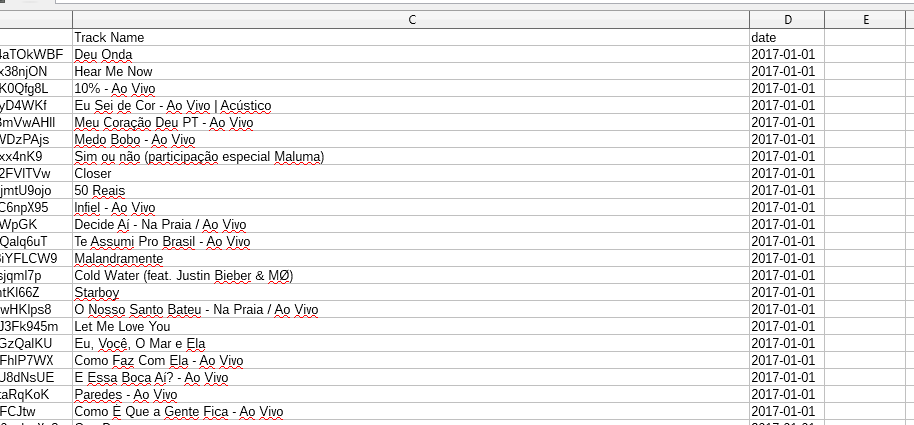
\includegraphics[width=\textwidth,height=\textheight,keepaspectratio]{../figs/parsed_charts_view.PNG}
\label{f.parsed_charts_view}
\legend{\small Fonte: Elaborada pelo autor.}
\end{figure}


\subsection{Coleta de indicadores econômicos}
\label{c.coleta_economicos}

Com as informações das músicas já obtidas e tratadas, passou-se à pesquisa sobre dados e indicadores de economia. Foi decidido, pela simplicidade e disponibilidade das informações, utilizar as métricas: Taxa Selic ("Sistema Especial de Liquidação e de Custódia", representa a taxa de juros) ~\cite{selic}, variação do IPCA ("Índice Nacional de Preços ao Consumidor Amplo", índice inflacionário oficial) ~\cite{ipca} e renda familiar média, disponível pelo PNAD, ou Pesquisa Nacional por Amostra de Domicílios ~\cite{pnad}. A pesquisa inicial pelos indicadores se deu pelo portal brasileiro de dados abertos oficial do governo ~\cite{dadosgov}, por onde os dados foram obtidos diretamente (por \textit{download} do arquivo) ou através do sistema referenciado no portal. No nosso caso, os dados sobre a taxa Selic foram obtidos pelo primeiro método, e os demais por meio do segundo. No caso, o sistema direcionou à base do Sistema IBGE de Recuperação Automática (SIDRA) ~\cite{sidra}, portal oficial que armazena dados provenientes das pesquisas do IBGE (Instituto Brasileiro de Geografia e Estatística). Por meio dele, foram referenciadas as tabelas das pesquisas apropriadas, PNAD para a renda média e IPCA para o próprio indicador, e selecionou-se os índices e períodos pertinentes.
No caso dos indicadores, foi adotado tratamento manual dos arquivos obtidos, visto que em sua maioria eram correções mais simples sem recorrer a um automatizador, e que compreendiam um número baixo de dados. No caso da tabela sobre a taxa Selic, não foi possível filtrar o intervalo de tempo que nos era interessante (2017-2018), sendo necessária a remoção das tuplas das datas fora da faixa de tempo. No caso das outras duas tabelas, o sistema SIDRA exportou os dados em um formato altamente estilizado, apresentando os dados de maneira que o interpretador do Pandas não era capaz de reconhecer e incluindo diversas outras informações irrelevantes ao contexto do algoritmo, como legendas. Assim, foi nescessário reorganizar os dados e remover as entradas decorativas das tabelas. Por fim, como a referência para a junção dos dados seria por data, os formatos das datas listadas nessas tabelas tiveram que ser retrabalhados, adaptando o formato brasileiro ("dia/mês/ano") usado nessas tabelas para o formato "ano-mês-dia", mais comum no contexto de tecnologia e usado nas listas de músicas, para facilitar a união dos dados.

\subsection{Análise de recursos de áudio}
\label{c.analise_audio}

Os dados coletados sobre as músicas até esse ponto não apresentavam relevância para o que esse projeto se propôs: isto é, não continham dados descritivos das qualidades musicais e de áudio das faixas para análise. Para tanto, valeu-se então da API oficial do \textit{Spotify}. Dentre os recursos de acesso disponibilizados pelo serviço, é de maior interesse o recurso de \textit{Audio Features}, ou recursos de áudio, das faixas. Esse \textit{endpoint}, dados um ou mais códigos de identificação, nos retorna uma análise com várias características musicais das obras consultadas, como a escala usada na composição, o tempo ou número de pulsos por minuto que determinam o andamento e velocidade da música, etc.

Para obter essas informações para cada entrada de dados das nossas músicas foi escrito um \textit{script Python} que importa os dois arquivos contendo as listas de músicas tratadas, realiza a união de suas tuplas, e para cada 50 entradas realiza uma chamada para a API do serviço, conforme o algoritmo~\ref{a.algoritmo_importa_audio}:

\begin{nicealgo}{a.algoritmo_importa_audio}
\naTITLE{Algoritmo de Importação de Recursos de Áudio}
\naPREAMBLE
\naINPUT{Tabela de Músicas 2017 T1 = [id1,id2,...,idn] e Tabela de Músicas 2018 T2 = [id1,id2,...,idm].}
\naBODY
\naBEGIN{}
	\na{\textbf{Seja} Tabela Geral T3 = T1 U T2;}
	\naBEGIN{\textbf{Para cada} tuplas $t$ em T3, \textbf{faça}}
		\naBEGIN{\textbf{Se} $t$ contém \textbf{nulo}, \textbf{então}}
		\naEND{\textbf{Elimina} $t$}
	\naEND{}
	\na{\textbf{Seja} Conjunto de recursos das músicas R = [];}
	\naBEGIN{\textbf{Para cada} 50 tuplas $t$ em T3, \textbf{faça}}
		\na{\textbf{Seja} Lista de recursos de uma música vi = [propriedade1, propriedade2,...,propriedaden];}
		\na{\textbf{Importe} Análise de áudio r = [v1,v2,...,v50]}
		\na{\textbf{Acrescente} $r$ ao final de $R$;}
	\naEND{}
	\na{\textbf{Exporte} $R$ \textbf{como} arquivo;}
\naEND{}
\end{nicealgo}

Desse modo, gera-se um novo arquivo, contendo as informações das propriedades sonoras disponíveis para análise pelo \textit{Spotify} de todas as músicas indexadas. As chamadas \textit{http} para o \textit{endpoint} relevante à obtenção dos dados foram realizadas com auxílio do pacote \textit{Spotipy}, que fornece uma interface simplificada para programas \textit{Python} interagirem com a API em questão.

\subsection{União dos dados de áudio com os \textit{sets} econômicos}
\label{c.uniao_economia_audio}

A última etapa no tratamento dos \textit{datasets} antes de poder passar à análise propriamente dita foi a união dos dados de índices econômicos com o recém gerado conjunto de atributos das faixas. Nesse ponto do projeto o desafio foi o de unir os arquivos de maneira a alinhar as datas corretamente. Isso porque, apesar de a taxa Selic e as faixas terem registros com precisão do dia, os dados de renda média e IPCA apenas registram variações mensais. Além disso, mesmo dentro do conjunto da tabela sobre a taxa Selic há várias entradas de dias faltantes, o que gera uma incorrespondência com as músicas desse período. Assim, o algoritmo deveria indexar os dados econômicos de 3 arquivos separados de acordo não apenas de acordo com a equivalência do dia da análise, mas também com a do mês dependendo da tabela sendo cruzada, além de considerar e tratar entradas nulas.

A primeira versão da rotina está descrita no algoritmo~\ref{a.algoritmo_1_mescla_dados}.

\begin{nicealgo}{a.algoritmo_1_mescla_dados}
\naTITLE{Algoritmo de Importação de Recursos de Áudio}
\naPREAMBLE
\naINPUT{Tabela de recursos de áudio T1 (onde $ti$ é uma tupla de dados) = [t1,t2,...,tn], Conjunto de tabelas de índices econômicos T2 (onde u1 é o conjunto de dados representando variação do IPCA, u2 a renda média e u3 a taxa Selic) = [u1,u2,u3]}
\naBODY
\naBEGIN{}
	\naBEGIN{\textbf{Para cada} tuplas $t$ em T1, \textbf{faça}}
		\na{\textbf{Seja} T3 = um conjunto vazio [];}
		\na{\textbf{Seja} d1 = dia da análise do áudio, em formato "yyyy-mm-dd";}
		\na{\textbf{Seja} d2 = primeiro dia do mês da análise do áudio, em formato "yyyy-mm-dd";}
		\naBEGIN{\textbf{Para cada} tabela $u$ em T2, \textbf{faça}}
			\naBEGIN{\textbf{Para cada} tupla $v$ em $u$;}
				\naBEGIN{\textbf{Se} $u['data']$ = $d1$ \textbf{ou} $u['data']$ = $d2$}
					\na{\textbf{Acrescente} $u$ ao final de $T3$;}
				\naEND{}
			\naEND{}
		\naEND{}
		\naBEGIN{\textbf{Para cada} tuplas $x$ em T3}
			\na{\textbf{Seja} i = Índice de iteração de T3;}
			\naBEGIN{\textbf{Se} $x$ \textbf{Contém nulo}}
				\na{\textbf{Seja} $c$ = coluna da célula de valor nulo;}
				\na{\textbf{Seja} f = próximo valor não nulo em $c$;}
				\na{\textbf{Seja} b = último valor não nulo em $c$;}
				\naBEGIN{\textbf{Se existe} T3[i+1]}
					\na{\textbf{Atribua} $x[c]$ = $f$;}
				\naEND{\textbf{Senão, atribua} $x[c]$ = $b$}
			\naEND{}
		\naEND{}
		\na{\textbf{Acrescente} a primeira tupla $x1$ de T3 a $t$;}
	\naEND{}
	\na{\textbf{Exporte} T1 \textbf{como} arquivo;}
\naEND{}
\end{nicealgo}

No entanto, o mesmo apresentou problemas severos de performance (como pode ser deduzido pelo npumero de iterações aninhadas) e resultados inconsistentes, principalmente devido a problemas com o algoritmo de concatenação do \textit{Pandas} para unir os resultados de pesquisa. Assim, foi trabalhada uma nova versão do programa, rodando um algoritmo com menos código e que, usando mais recursos prontos de otimização do \textit{Python} e \textit{Pandas}, conseguiu fazer a mescla dos indicadores econônicos às informações de áudio das faixas de modo mais performático e com melhor consistência.

\begin{lstlisting}[language=Python, caption=Script de mesclagem entre os dados da análise de áudio e indicadores econômicos]
import config
from fycharts import SpotifyCharts
import pandas as pd
import numpy as np
import glob
from datetime import datetime as dt

def getMonthBegin(date):
	monthBegin = dt.strptime(date,'%Y-%m-%d')
	monthBegin = dt(monthBegin.year,monthBegin.month,1)
	return dt.strftime(monthBegin,'%Y-%m-%d')

def matchValueByDate(date1,date2,df,col):

	matchId = np.where(date1.values == date2)[0]
	if matchId.size == 0 and col != 'daily_rate':
		date2 = getMonthBegin(date2)
		matchId = np.where(date1.values == date2)[0]
		if matchId.size == 0:
			return None

	if col == 'daily_rate' and matchId.size == 0:
		return None
	else:
		val = df.loc[matchId[0],col]
	return val

def generateTableset(country):
	audioFeats = pd.read_csv(config.DATA['output_path']+'/'+country+'/audio-features.csv')
	econTables = fetchEconomicData(country)
	ecoData = []

	for df in econTables:
		cols = list(df)
		for col in cols:
			if(col == 'date'):
				continue
			audioFeats[col] = audioFeats.apply(lambda row: matchValueByDate(df['date'],row['date'],df,col),axis=1)

	print("NEW SET: \n {}".format(audioFeats));
	audioFeats.to_csv(config.DATA['output_path']+'/'+country+'/audio-economic-features.csv')

def fetchEconomicData(country):
	econFiles = glob.glob(config.DATA['data_path']+'/economics/'+country+'/*')
	econTables = []
	for file in econFiles:
		df = pd.read_csv(file,index_col=[0])
		econTables.append(df)
	return econTables
\end{lstlisting}

Apesar de, à primeira vista, haver indicadores de que a performance seria similiar entre ambos, como são usados recursos mais otimizados do \textit{Pandas} para as iterarações na tabela de parâmetros sonoros e não serem realizadas tantas operações de concatenação entre tuplas e tabelas já reduziu a maior parte do tempo de execução inicial. Após averiguação da tabela gerada e algumas correções no algoritmo, passou-se à análise propriamente dita usando o arquivo gerado.

\section{Algoritmo de análise}
\label{c.analise_alg}

Paralelamente à criação dos \textit{scripts} para gerar e tratar as tabelas de dados foi construído o conjunto de algoritmos para pré-processar e executar a análise dos dados. Até que os \textit{datasets} tratados ficassem prontos, para fins de teste do \textit{software} foram usados conjuntos prontos (como os vindos do pacote \textit{scikit-learn}, ou de outras fontes como o Kaggle), ou partes das tabelas já obtidas (como a tabela de análise de áudio assim que o \textit{crawler} ficou pronto). O trabalho dividiu-se primariamente em organizar um pré-processador, a execução propriamente dita da análise (treinamento e teste do algoritmo) e retorno dos resultados.

\subsection{Pré processador}
\label{c.preprocessor}

O objetivo do pré-processador foi o de encontrar os melhores parâmetros para desempenho do regressor e preparar os dados para a análise final. Dentro da preparação dos dados, o primeiro passo foi eliminar as entradas nulas dos dados de análise e do conjunto alvo a ser previsto. Apesar de esse tratamento já ter sido aplicado em diversas etapas do processamento e agrupamento dos dados, a tabela final ainda não havia sido tratada, sendo necessário passar a esse passo, já que entradas nulas poderiam, na melhor das hipóteses, viciar ou interferir nos resultados, e na pior, causar erros no algoritmo, forçando sua parada.

Passada essa primeira etapa, foram removidas as colunas inconsequentes ou danosas à análise. Como o objetivo era uma predição de características musicais baseada em índices econômicos, dados como o identificador e data de coleta podem e devem ser ignorados para não interferirem de alguma forma nos resultados. Da mesma forma, deve-se eliminar o conjunto a ser calculado da lista de índices econômicos, colocando-o em uma variável separada que, para fins de clarificação, será referida daqui para frente como \textit{target}. Isso porque, do contrário, corre-se o risco de viciar o preditor a usar a própria entrada como parâmetro de previsão, nos dando resultados falsamente precisos. O \textit{target}, e consequentemente as colunas a serem separadas, foi selecionado de maneira diferente para experimentação, de modo que o processo estará descrito com maior clareza nessa seção do trabalho.

Por fim, passou-se ao seletor de parâmetros. O método usado para o treino do modelo e predição dos atributos das faixas, o SVR (\textit{Support Vector Regressor}) já veio integrado à biblioteca \textit{scikit-learn}, mas apesar dessa conveniência ainda era necessário ajustar o conjunto de parâmetros usado pela função, bem como o \textit{Scaler} usado. Para o algoritmo usado, os parâmetros para ajuste mais interessantes são: \textit{kernel} (algoritmo de manipulação dos dados para uso na SVM), \textit{C} (parâmetro de punição de erros, para controle de rigidez nos resultados), e \textit{gamma} (parâmetro de controle de viés dos dados). O processo de seleção se deu como descrito pelo algoritmo~\ref{a.algoritmo_seletor_params_svm}:

\begin{nicealgo}{a.algoritmo_seletor_params_svm}
\naTITLE{Algoritmo de Seleção de Parâmetros para SVR}
\naPREAMBLE
% \naINPUT{Conjunto do \textit{target} T = [t1,t2,...,tn] e Conjunto de indicadores para regressão R = [r1,r2,...,rn]}
\naBODY
\naBEGIN{}
	% \na{\textbf{Seja} Y = Subconjunto aleatório de T com 75\% dos dados e y = T-Y;}
	% \na{\textbf{Seja} X = Subconjunto aleatório de R com 75\% dos dados e x = R-X;}
	\na{\textbf{Seja} M o modelo de regressão (SVR)}
	\na{\textbf{Seja} lista de Kernels padrão do \textit{scikit-learn}: K = ['rbf','linear','poly','sigmoid'];}
	\na{\textbf{Seja} lista de valores para parâmetro C: C = [0.001,0.01,0.1,1,10,100];}
	\na{\textbf{Seja} lista de valores para parâmetro Gamma: G = [0.001, 0.01, 0.1, 1, 10, 100];}
	\na{\textbf{Seja} n = o número de combinações a ser testado;}
	\na{\textbf{Seja} H = conjunto de resultados do coeficiente de determinação r²;}
	\na{\textbf{Seja} Conjunto de parâmetros B = [];}
	\naBEGIN{\textbf{Para n} combinações $b$ de $K$, $C$ e $G$, \textbf{faça}}
		\na{\textbf{Treine} M com os parâmetros $b$;}
		\na{\textbf{Seja} h = coeficiente de determinação r² de $M(b)$;}
		\na{\textbf{Acrescente} h a H;}
		\naBEGIN{\textbf{Se} h = \textbf{Máximo} em H}
			\na{B = $b$}
		\naEND{}
	\naEND{}
	\na{\textbf{Retorne} B;}
\naEND{}
\end{nicealgo}

Para realizar a parte de combinação de parâmetros e treinamento/teste do modelo foi inicialmente utilizada a classe \textit{GridSearchCV} do \textit{scikit-learn}. Entretanto, principalmente ao tentar operações com \textit{targets} compostos por múltiplas colunas de dados, a performance da mesma caiu drasticamente. Optou-se por um pacote similar chamado \textit{BayesSearchCV} de um projeto filho: o \textit{scikit-optimize}, após verificar melhora no tempo de execução. Apesar de ainda ser um processo lento e oneroso, foi necessário para maximizar a precisão dos resultados. Um fluxo similar foi aplicado para os \textit{scalers}, onde testou-se apenas dois dos mais comuns: o \textit{StandardScaler} e o \textit{MinMaxScaler}. São treinados dois modelos usando o mesmo conjunto de dados e método de análise e retorna-se o mais bem sucedido de acordo com o coeficiente de determinação ($R^2$)~\ref{t.regression_metrics}.

Apesar da carga de processamento e tempo gasto, os procedimentos acima foram aplicados diversas vezes, para ajustar o modelo a diferentes conjuntos de \textit{targets} e, por consequente, de dados de análise.

\subsection{Visualização dos resultados}
\label{c.visualizador}

Por fim, foi escrito um conjunto pequeno de rotinas para exibição das métricas de desempenho dos modelos gerados. Os indicadores escolhidos foram: indicador de variação explicada, erro médio absoluto, erro quadrado médio, erro médio quadrado logarítmico, desvio mediano absoluto e coeficiente de determinação, ou $R^2$~\ref{t.regression_metrics}. As funções simplesmente exibem o valor de cada um no terminal baseado na predição de um modelo determinado. Apesar de ser mais "cru", foi um indicador visual suficiente para avaliar o desempenho do algoritmo para diferentes parâmetros, \textit{sets} de dados e \textit{targets}.

\section{Experimentação e resultados}
\label{c.experimentacao}

Por fim passou-se à fase de experimentação. O objetivo dessa etapa foi testar diversas combinações de \textit{targets} para determinar o modelo com previsão mais precisa e, portanto, quais os conjuntos características de áudio o algoritmo melhor consegue prever. Foi escrito um \textit{script} simples para acessar o pré processador e, com o modelo retornado, executar o treino e teste, exibindo posteriormente os desvios descritos acima.

As características das músicas a serem estimadas e suas descrições são como detalhado pela tabela~\ref{t.audio_features_desc}, montada a partir da documentação oficial da API do \textit{Spotify}.

\begin{tabularx}{\linewidth}{c|X}
\caption{Descrição das características da análise de áudio}\label{t.audio_features_desc}\\
\toprule
\textbf{Nome do campo} & \textbf{Descrição}\\[6pt]
\midrule
\endhead
	{duration\_ms} & {Duração da faixa em milissegundos(ms).}\\\hline
	{key} & {Tom estimado em que a faixa foi composta. É mapeada por números inteiros de acordo com notação numérica americana, onde 0 equivale à nota dó, 1 equivale a dó sustenido/ré bemol, e assim por diante até a nota si, que equivale ao numeral 11. Caso não haja estimativa do tom, é usado o valor -1.}\\\hline
	{mode} & {Indicador da modalidade (maior ou menor) predominante na melodia da faixa. O número 1 representa modalidade maior e o 0, menor.}\\\hline
	{time\_signature} & {A notação de tempo estimada como predominante da faixa. É uma convenção do número de pulsos (batidas) em um ciclo da música (compasso).}\\\hline
	{acousticness} & {Um gradiente de confiança de 0 a 1 do quão "acústica" (isto é, o quão ausentes são elementos eletrônicos como: distorções, \textit{MIDI}, etc. na sua composição, gravação ou produção) é uma faixa, onde 1 representa alta confiança da faixa ser "acústica" e 0, baixa confiança.}\\\hline
	{danceability} & {Gradiente de 0 a 1 descrevendo o quão adequada a música é para dançar, baseado em uma combinação de elementos da música como: tempo, estabilidade rítmica, força do pulso (ou batida), e regularidade em geral. O número 0 representa baixa adequação à dança, e o 1, alta.}\\\hline
	{energy} & {Medidor de 0 a 1 que representa a medida de intensidade e atividade percebidas na música. Tipicamente, faixas com maior "energia" são mais rápidas e barulhentas e são atribuídas um valor mais próximo de 1, enquanto a faixas "calmas" atribui-se um índice mais próximo de 0. Fatores perceptuais que afetam esse atributo incluem: variedade na dinâmica (ou intensidade sonora) da peça, sonoridade percebida, timbre, toada inicial e entropia em geral.}\\\hline
	{instrumentalness} & {Preditor se uma música contém ou não elementos vocais, isto é, com uso de voz humana (considera-se apenas a dicção clara de palavras, fonemas simples e isolados são desconsiderados). Quanto mais próximo o valor é de 1, maior a probabilidade de a obra não conter conteúdo de voz humana. Valores acima de 0.5 pretendem representar obras instrumentais, mas índices mais próximos de 1 inferem maior confiança na medição.}\\\hline
	{liveness} & {Detecta a presença de uma audiência "ao vivo" na gravação, representado em um gradiente de 0 a 1. Valores mais próximos de 1 representam maior probabilidade de uma faixa ter sido gravada com um público espectador.}\\\hline
	{loudness} & {A sonoridade geral de uma faixa, medida em decibeis (dB). Os valores constituem uma média da intensidade sonora de toda a gravação, e é usada para comparar a sonoridade relativa entre músicas. Os valores típicos se encontram entre -60dB e 0dB}\\\hline
	{speechiness} & {Intervalo de 0 a 1 que representa a confiança de uma faixa apresentar elementos de palavra falada, isto é, de não ser apenas instrumental. Quanto menos elementos musicais além da voz, mais próximo de 1 e valores acima de 0.66 tendem a representar faixas exclusivamente com texto declamado, sem demais elementos musicais ou instrumentos. Valores entre 0.33 e 0.66 representam em geral faixas híbridas e abaixo de 0.33, música ou outros formatos não discursivos.}\\\hline
	{valence} & {Uma métrica de 0 a 1 descrevendo a "positividade" da música, com maior valência representando músicas mais "positivas" (ex.: eufóricas, alegres, animadas) e menor, mais "negativas" (ex.: triste, deprimente, irada).}\\\hline
	{tempo} & {O tempo médio estimado de uma faixa, em batidas por minuto(bpm). Na terminologia musical, o tempo de uma composição representa sua velocidade ou andamento e deriva diretamente da duração média da batida.}\\\hline
	\bottomrule
	
\end{tabularx}

Para avaliação a performance do preditor foi utilizado um conjunto de métricas de erro próprias para algoritmos de regressão. Sua descrição se encontra na tabela~\ref{t.regression_metrics}.

\begin{tabularx}{\linewidth}{c|X}
\caption{Métricas de avaliação do algoritmo de regressão.}\label{t.regression_metrics}\\
\toprule
\textbf{Métrica} & \textbf{Descrição}\\[6pt]
\midrule
\endhead
	{Indicador de variação explicada} & {Mede a proporção em que o modelo considera a dispersão (ou variância) de um conjunto de dados. Tenha que $\widehat{y}$ é o valor de saída alvo, $y$ é o valor de saída real e $Var$ é a variância (quadrado do desvio padrão), a variância explicada $V$ é expressa por: $V(y,\widehat{y}) = 1 - \frac{Var\{y-\widehat{y}\}}{Var\{y\}}$. Melhor valor possível é 1.}\\\hline

	{Erro médio absoluto} & {Valor médio absoluto esperado para o erro. Tenha que $\widehat{y}_i$ é o valor previsto da $i$-ésima amostra e $y_i$ é o valor real observado, o erro (EMA) estimado sobre $n$ amostras é expresso por: $EMA(y,\widehat{y}) = \frac{1}{n} \sum_{i=0}^{n-1} |y_i-\widehat{y}_i|$. Melhor valor possível é 0. Não admite valores negativos.}\\\hline

	{Erro quadrado médio} & {Valor médio esperado para o erro quadrático. Atribui maior peso a erros maiores e menor peso a erros menores. Tenha que $\widehat{y}_i$ é o valor previsto da $i$-ésima amostra e $y_i$ é o valor real observado, o erro (EMQ) estimado sobre $n$ amostras é expresso por: $EMQ(y,\widehat{y}) = \frac{1}{n} \sum_{i=0}^{n-1} (y_i-\widehat{y}_i)^2$. Melhor valor possível é 0. Não admite valores negativos.}\\\hline

	{Erro quadrado médio logarítmico} & {Valor esperado para o quadrado da transformação logarítmica do erro. Atribui maior peso a erros maiores e menor peso a erros menores. Tenha que $\widehat{y}_i$ é o valor previsto da $i$-ésima amostra e $y_i$ é o valor real observado, o erro (EQML) estimado sobre $n$ amostras é expresso por: $EQML(y,\widehat{y}) = \frac{1}{n} \sum_{i=0}^{n-1} (\log_{e}{(y_i + 1)}-\log_{e}{(\widehat{y}_i+1)})^2$, onde $\log_{e}{x}$ é o logaritmo natural de $x$. essa métrica é melhor adequada para modelos de crescimento exponencial. Como nota de atenção, ela também penaliza subestimativas mais do que sobrestimativas nas previsões. Melhor valor possível é 0. Não admite valores negativos.}\\\hline

	{$R^2$} & {Também chamado coeficiente de determinação. Representa a proporção da variância explicada pelas variáveis independentes do modelo. Provê um incador da adequação e, assim, a medida do quão bem amostras ainda não analisadas serão previstas pelo modelo por meio da proporção da variância explicada. Tenha que $\widehat{y}_i$ é o valor previsto da $i$-ésima amostra, $y_i$ é o valor real observado, $\overline{y} = \frac{1}{n} \sum_{i=1}^{n}\widehat{y}_i$ e $\sum_{i=1}^{n} (y_i-\widehat{y}_i)^2 =  \epsilon_i^2$, o $R^2$ estimado sobre $n$ amostras é expresso por: $R^2(y,\widehat{y}) = 1 - \frac{\sum_{i=1}^{n} (y_i-\widehat{y}_i)^2}{\sum_{i=1}^{n} (y_i-\overline{y})^2}$. Melhor valor possível é 1 e pode retornar valores negativos. Um modelo constante que sempre prediz o valor esperado de $y$, independente das características de entrada possui valor 0.}\\\hline
	\bottomrule
\end{tabularx}
\legend{Fonte: ~\cite{scikitlearn_api_doc_regression}}

O primeiro teste foi sobre o conjunto de todas as características de áudio como \textit{target}, isto é, o modelo tenta prever todos os parâmetros baseado nos indicadores econômicos. Os resultados foram como descrito na figura~\ref{f.params_all_audio_features} e tabela ~\ref{t.params_all_audio_features}.

\begin{figure}[H]
	\caption{Resultados de predição de todos os atributos de áudio.}
	\centering
	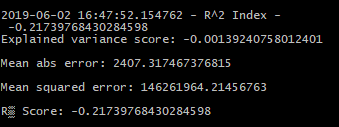
\includegraphics[width=\textwidth,height=\textheight,keepaspectratio]{../figs/params_all_audio_features.PNG}
	\label{f.params_all_audio_features}
	\legend{Fonte: Elaborada pelo autor.}
\end{figure}

\begin{table}[H]
	\centering
	\caption{Resultados de predição de todos os atributos de áudio.}\label{t.params_all_audio_features}
	\begin{tabular}{c|c}
		\hline
		\textbf{Métrica} & \textbf{Resultado}\\\hline \hline
		{Indicador de variação explicada} & {\~- -0,0014}\\\hline
		{Erro médio absoluto} & {\~- 2407,3175}\\\hline
		{Erro quadrado médio} & {\~- 146261964,2146}\\\hline
		{R²} & {\~- -0,2174}\\\hline
	\end{tabular}
	\legend{Fonte: Elaborada pelo autor.}
\end{table}

Como observado, o erro calculado para todas as métricas foi grande, retornando assim resultados insatisfatórios. Uma das possíveis razões foi a inadequação do algoritmo de regressão escolhido para operar com o número de variáveis (treze no total) a ser previsto. Experimentou-se então o extremo oposto, construindo um \textit{target} com apenas uma variável. A variável escolhida foi a \textit{valence}, ou valência. A escolha do parâmetro se deu por duas razões: sua ligação direta com a qualidade das emoções percebidas; seu cálculo, que por ser feito a partir de diversos outros atributos, abre a possibilidade de que eles sejam adequadamente representados por esta única variável. Os novos resultados estão descritos na figura~\ref{f.params_valence_feature} e tabela ~\ref{t.params_valence_feature}.

\begin{figure}[H]
\caption{Resultados de predição da valência.}
\centering
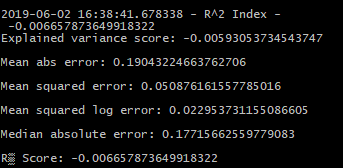
\includegraphics[width=\textwidth,height=\textheight,keepaspectratio]{../figs/params_valence_feature.PNG}
\label{f.params_valence_feature}
\legend{Fonte: Elaborada pelo autor.}
\end{figure}

\begin{table}[H]
\centering
\begin{tabular}{c|c}
\hline
\textbf{Métrica} & \textbf{Resultado}\\\hline \hline
{Indicador de variação explicada} & {\~- -0,0059}\\\hline
{Erro médio absoluto} & {\~- 0,1904}\\\hline
{Erro quadrado médio} & {\~- 0,0509}\\\hline
{Erro quadrado médio logarítmico} & {\~- 0,0229}\\\hline
{R²} & {\~- -0,0067}\\\hline
\end{tabular}
\caption{Resultados de predição da valência.} \label{t.params_valence_feature}
\legend{Fonte: Elaborada pelo autor.}
\end{table}

Apesar dos parâmetros R² e de variação explicada exporem que o modelo não é o mais adequado, os resultados dos demais erros foram satisfatórios, com erro médio baixo em todos as medições. No entanto, por ser um valor calculado discretamente pelo serviço do \textit{Spotify}, não há prova empírica de que a valência representa os demais atributos omitidos. Assim, foi calculado um último teste, onde analisou-se apenas a tabela de recursos de áudio e tentou-se predizer a valência a partir das demais qualidades. Os resultados estão descritos na figura~\ref{f.test_valence_results} e tabela~\ref{t.test_valence_results}.

\begin{figure}[H]
\caption{Resultados de predição da valência baseado nos demais atributos das faixas.}
\centering
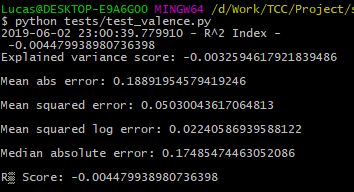
\includegraphics[width=\textwidth,height=\textheight,keepaspectratio]{../figs/test_valence_results.PNG}
\label{f.test_valence_results}
\legend{Fonte: Elaborada pelo autor.}
\end{figure}

\begin{table}[H]
\centering
\begin{tabular}{c|c}
\hline
\textbf{Métrica} & \textbf{Resultado}\\\hline \hline
{Indicador de variação explicada} & {\~- -0,0033}\\\hline
{Erro médio absoluto} & {\~- 0,1889}\\\hline
{Erro quadrado médio} & {\~- 0,0503}\\\hline
{Erro quadrado médio logarítmico} & {\~- 0,0241}\\\hline
{R²} & {\~- -0,0045}\\\hline
\end{tabular}
\caption{Resultados de predição da valência.}\label{t.test_valence_results}
\legend{\small Fonte: Elaborada pelo autor.}
\end{table}

Observa-se que os resultados foram similares aos obtidos acima. Apesar da baixa variação, que nos indica uma boa predição, infelizmente novamente constata-se pelos indicadores R² e de variação explicada que o modelo não é o mais adequado.